
\begin{document}

This section covers the design choices associated with the actively loaded differential amplifier with cascoded current mirror and a class B amplifier for an output stage. Frequency compensation will also be considered in the development to ensure stability.

The circuit that was developed in Task 4 will be used for the purposes of this circuit development section. The output stage will be added in this task which will be a class B amplifier. The class B amplifier will consist of a 2n3904 NPN BJT and a 2n3906 PNP BJT. The simulations were conducted in Microcap 10. As these schematics are difficult to read, a set of schematics with identical values and components were created in Eagle by Autodesk. The simulated schematic can be seen in Figure \ref{fig:simschem} below.

\begin{figure}[H]
	\centering
	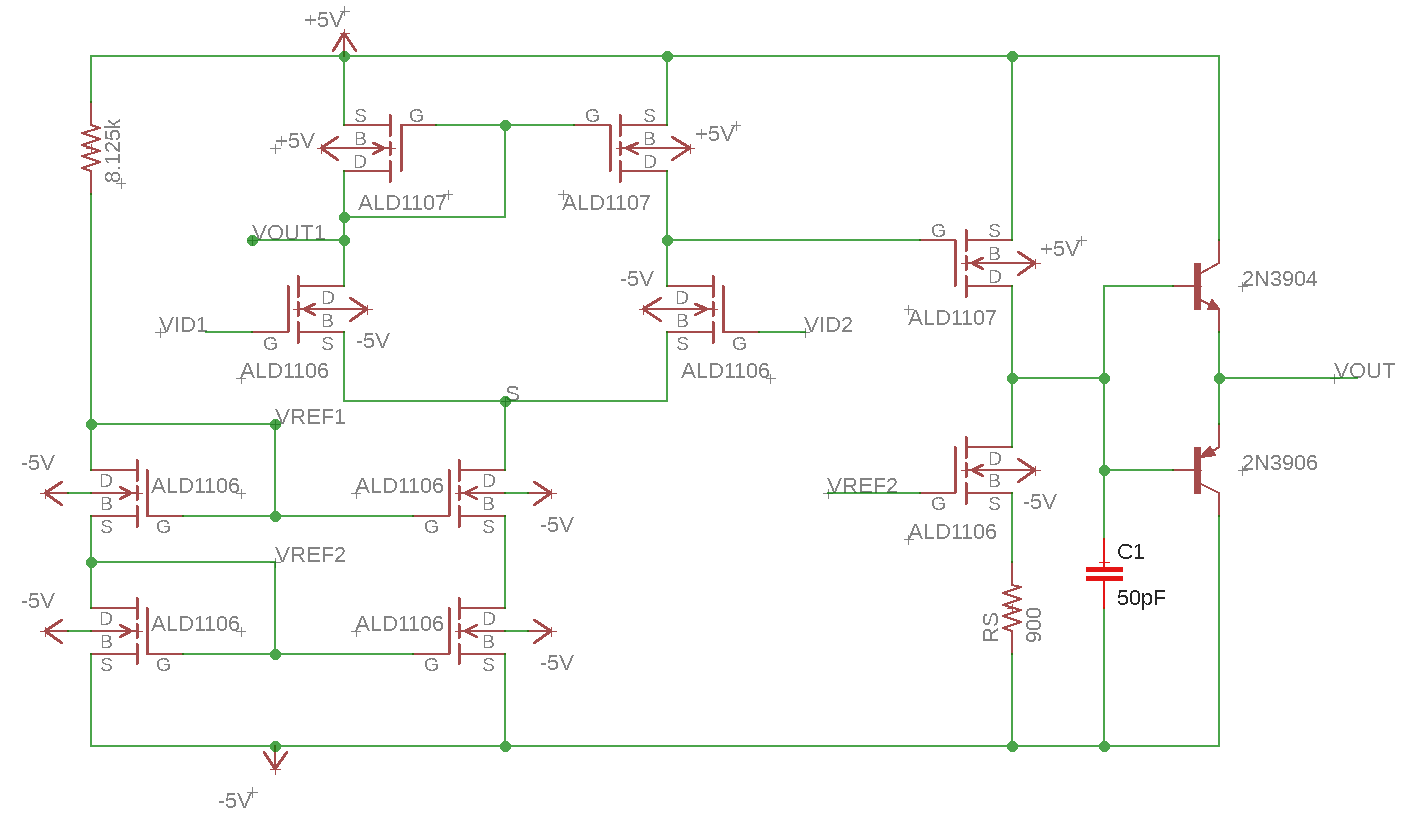
\includegraphics[width=0.8\linewidth]{CircuitDevelopment/schematicsimulation.png}
	\caption{Simulated Circuit}
	\label{fig:simschem}
\end{figure}

The value of 13 k$\Omega$ was unchanged from Task 4 which gave a reference current of 401 $\mu$A. There are several specifications to meet, or at least come near for the completion of this task. The unity gain frequency should be above 150 kHz. A small load resistance of 500 $\Omega$ or less should cause a drop of 3 dB from the unloaded gain. Lastly, the gain needs to be high than 200 V/V or 46 dB. The equation for closed loop gain is shown below in equation \ref{eqn:closedloop}.

\begin{equation}
A_f(j\omega) = \frac{x_o}{x_i} = \frac{A_f(j\omega)}{1+A_f(j\omega)\beta}
\label{eqn:closedloop}
\end{equation}

The part of the denominator, $A_f(j\omega)\beta$ is the actual loop gain for the amplifier, which it is much greater than one, then the closed loop gain is approximately $\frac{1}{\beta}$. The value of $\beta$ in this case was found to be 21$\frac{V}{V} $. The value for the resistor at the source of the ALD1106 NMOS, RS, was found to be 1.1k in the previous lab, and yielded similar results for this simulation, as it gave the appropriate offset nulling at the base of the BJTs at approximately zero volts. This will allow the amplifier to have it's maximum amount of gain. 

The output of the amplifier met the specifications as it was simulated to have a 63.3 dB gain. To find the smallest load resistor that the amplifier could drive, Microcap 11 was used to do a sweep of load resistor values from 250 $\Omega$ to 2.5 k$\Omega$. The goal is to find the load resistor value that will cause a 3 dB drop from the unloaded gain, which would be 60.3 dB, or at least a value close to that. The result can be seen in Figure \ref{fig:loadsweep} below.

\begin{figure}[H]
	\centering
	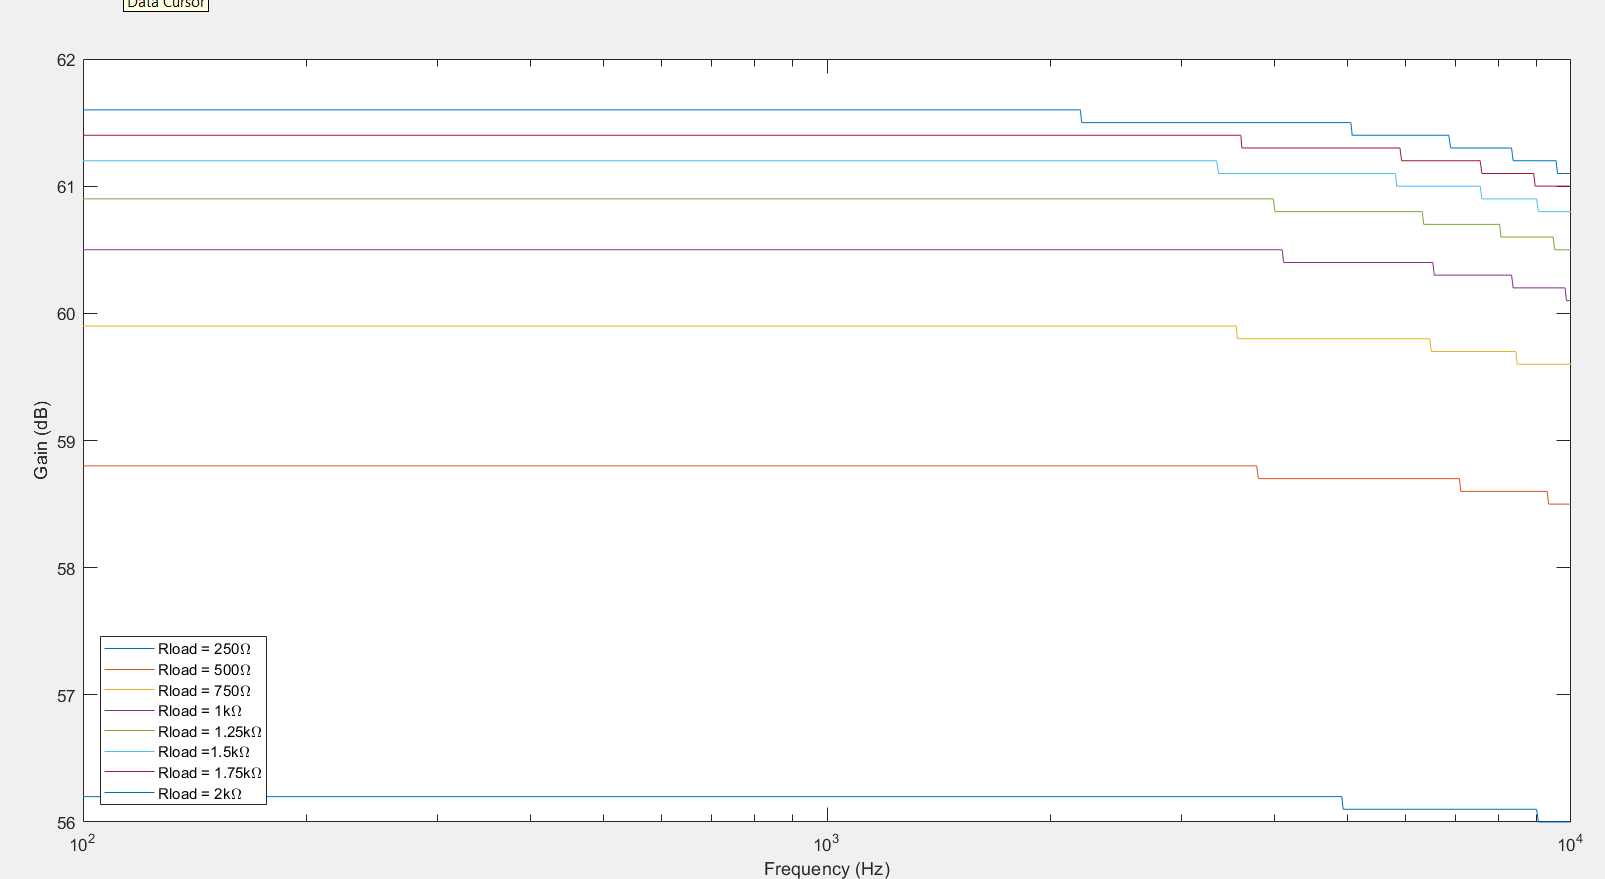
\includegraphics[width=0.7\linewidth]{CircuitDevelopment/varyrload.png}
	\caption{Sweep values of load resistor vs gain}
	\label{fig:loadsweep}
\end{figure}


It was found that the load of approximately 900 $\Omega$ caused a 3 dB drop in gain. A load of 500 $\Omega$ caused a 6 dB drop. Therefore, 900 is the smallest load the circuit can drive according to the simulation. Using this value for the load, a simulation was conducted and the resulting data was exported to Matlab to plot. The gain verses frequency plot at a 900 $\Omega$ load resistance is seen below in Figure \ref{fig:loadgain}. During this simulation, the capacitor at the collector of the 2n3906 (used for frequency compensation) was found to work at any value below 500 pF. 

\begin{figure}[H]
	\centering
	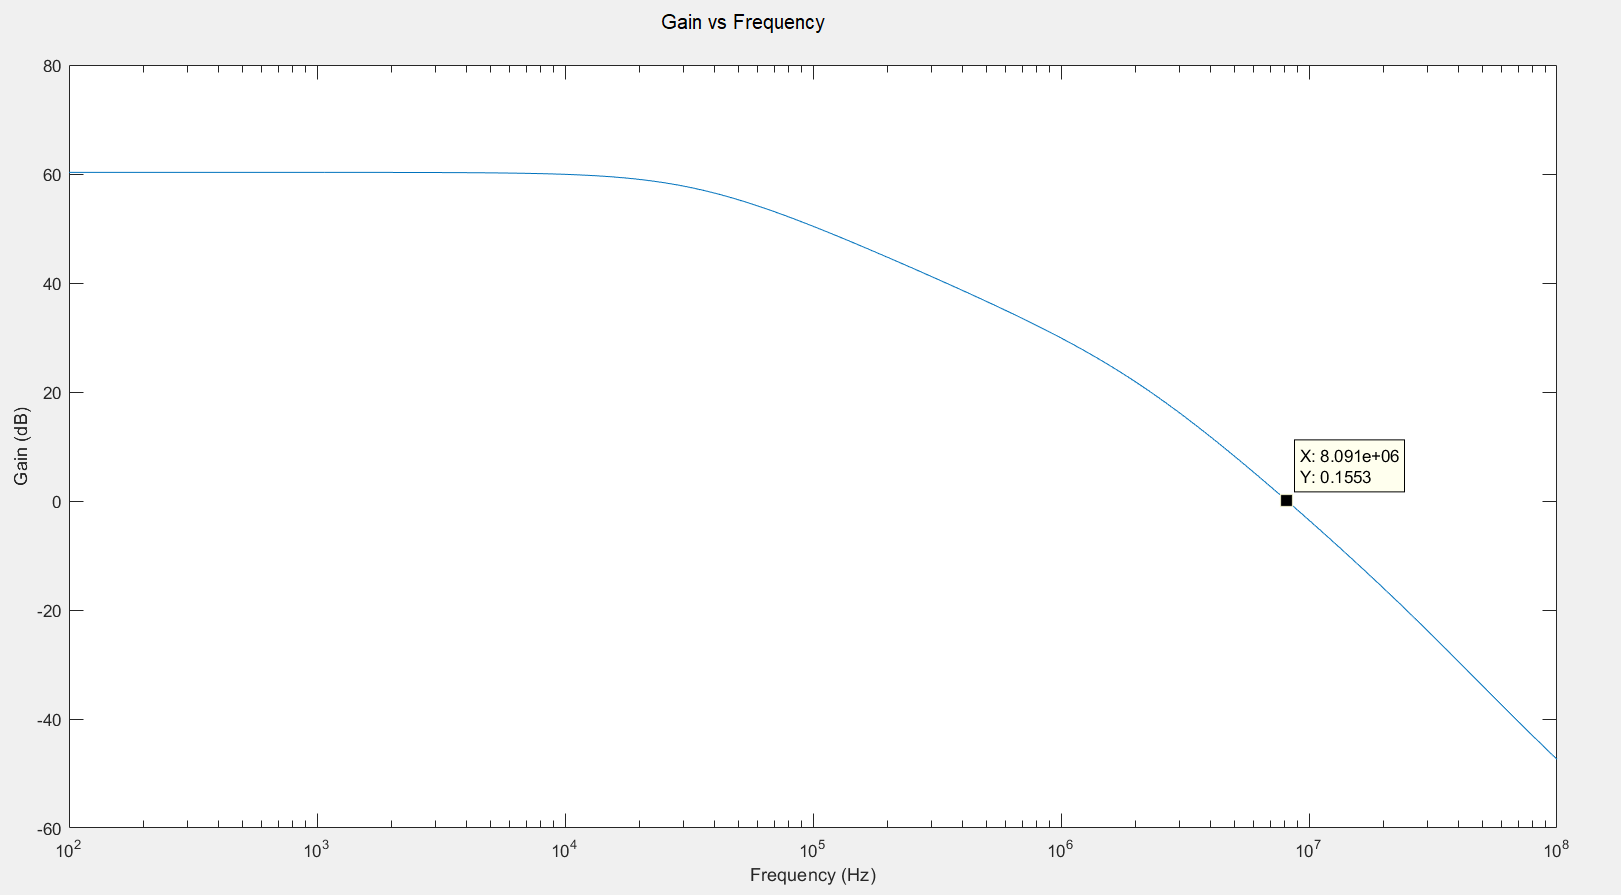
\includegraphics[width=0.7\linewidth]{CircuitDevelopment/gainfreqsim.png}
	\caption{Gain with 900 $\Omega$ load resistance}
	\label{fig:loadgain}
\end{figure}

As seen, the gain is valued at just over 60 dB, which meets the 3 dB drop in gain requirement at 900 $\Omega$ load. The zero crossing for the gain was found to be approximately 8 MHz. In order to be a stable amplifier, the phase shift should not change more than 180 degrees before the zero crossing of the gain. The resultant phase plot from simulations is see in Figure \ref{fig:phasesim} below.


\begin{figure}[H]
	\centering
	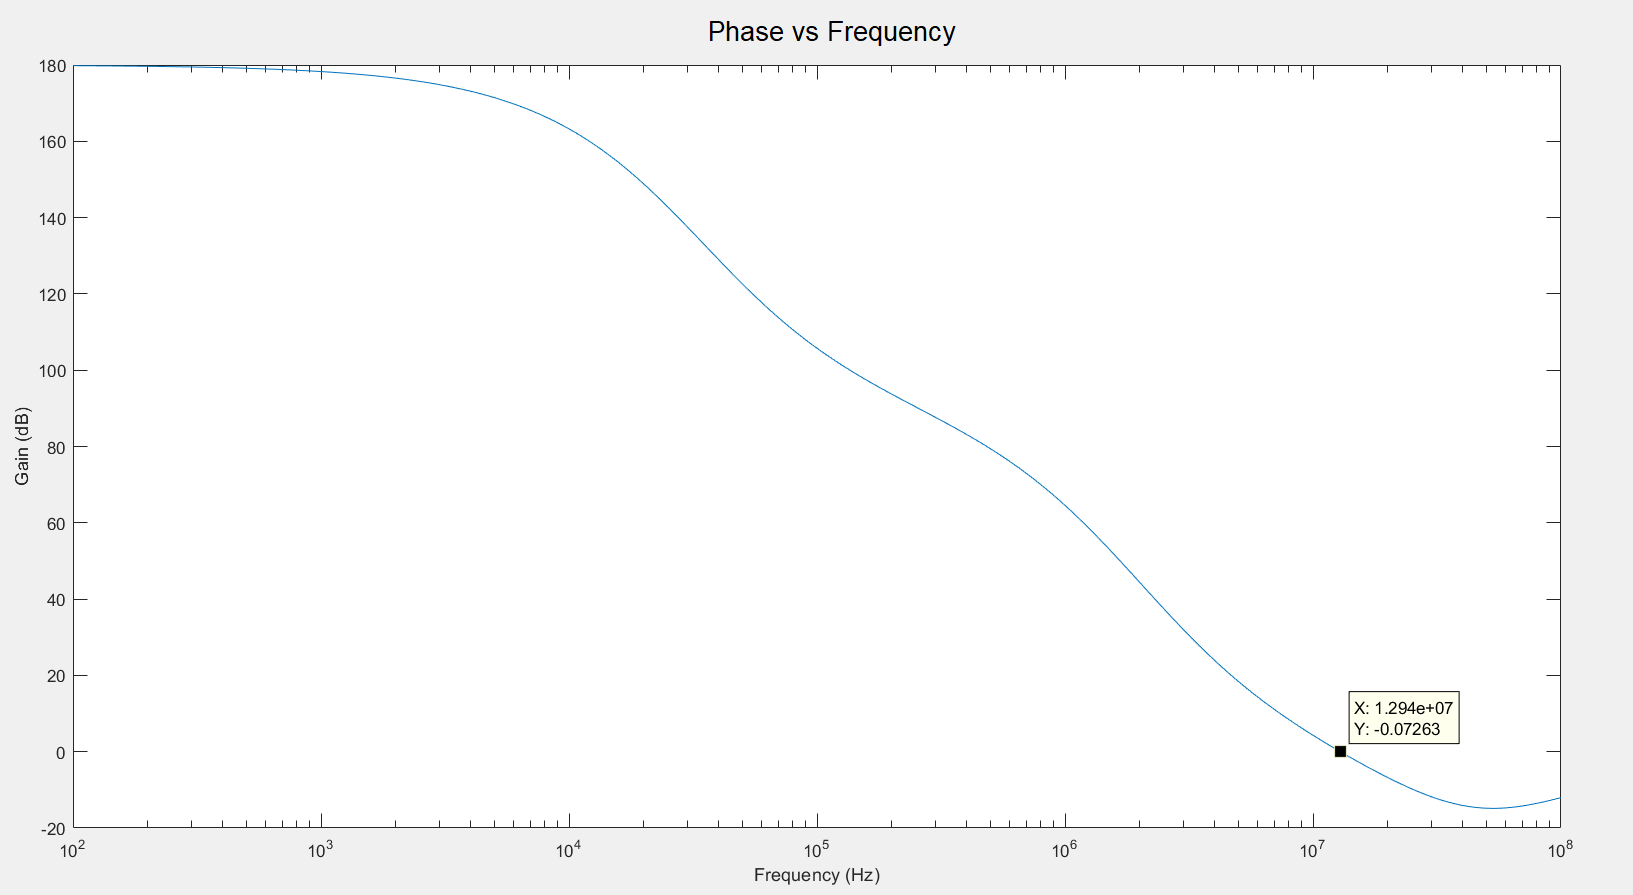
\includegraphics[width=0.7\linewidth]{CircuitDevelopment/phasefreqsim.png}
	\caption{Phase plot with 900 $\Omega$ load resistance}
	\label{fig:phasesim}
\end{figure}

The value for an 180 degree phase shift was found to be approximately 12.9 MHz from the simulations. This is well beyond the required 8.9 MHz found from the plot of the gain in Figure \ref{fig:loadgain}. All of the nodal voltages and currents were found during the simulation using dynamic DC analysis in Microcap 11. The current values are shown in Table \ref{tab:simcircuitcurrent} AC analysis was used in order to simulate the gain and phase. 


\begin{table}[H]
	\centering
	\caption{Current values from simulated circuit}
	\label{tab:simcircuitcurrent}
	\begin{tabular}{|l|c|}
		\hline
		\multicolumn{2}{|l|}{Simulated current values}                            \\ \hline
		I$_{Ref}$ & 410.8 $\mu$A                                                  \\ \hline
		I$_{D_1}$ & 204.4 $\mu$A                                                  \\ \hline
		I$_{D_2}$ & 204.4 $\mu$A                                                  \\ \hline
		I$_{CS}$  & $\approx$  227 $\mu$A                                         \\ \hline
		I$_{C}$   & $\approx$ 2  $\mu$A										 \\	\hline

	\end{tabular}
\end{table}

The voltage values are seen in Table \ref{tab:simcircuitvoltage} below. 

\begin{table}[H]
	\centering
	\caption{Current values from simulated circuit}
	\label{tab:simcircuitvoltage}
	\begin{tabular}{|l|c|}
		\hline
		\multicolumn{2}{|l|}{Simulated voltage values}                            \\ \hline
		V$_{Ref2}$ & -340 mV                                                  \\ \hline
		V$_{Ref1}$ & -2.987 V                                                 \\ \hline
		V$_{D_1}$ & 2.796 V                                                  \\ \hline
		V$_{D_2}$  & 2.796 V                                      \\ \hline
		V$_{Base}$   & 9.7 $\mu$V										 \\	\hline
		V$_{out}$ & $\approx$ 0 V \\ \hline
	\end{tabular}
\end{table}

The circuit simulated as expected with the chosen DC bias conditiions utilizing a bias current of 400$\mu$A.


\end{document}